\chapter{Forforstærker}
\label{forforstaerker}
Forforstærkerens opgave er, som nævnt i kapitel \ref{systemopbygning}, at forstærke et mikrofonsignal op til linieniveau. Ved gennemgangen af relevante standarder i afsnit \ref{standarder} ses det, at et liniesignal ligger med peakspændinger mellem 200 mV og 2 V, mens et mikrofonsignal ligger med peakspændinger mellem 0,8 mV og 200 mV. Der er altså for et liniesignal en faktor 10 mellem den laveste og den højeste signalspænding, mens der for et mikrofonsignal er en faktor 250 mellem de to yderpunkter. Denne forskel bevirker at signalet fra en mikrofon, hvis udgangssignal ligger i området beskrevet i standarden, ikke kan forstærkes lineært til linieniveau.\\ 
Givet at spændingen efter forforstærkeren må variere med en faktor 10, da den skal være på linieniveau, og forforstærkeren ønskes at forstærke lineært, må spændingen på indgangen af forforstærkeren også kun variere med en faktor 10. Eftersom denne spændingen bestemmes af lydtrykket på mikrofonen, må lydtrykket på mikrofonen altså variere med 20 dB(A), da dB(A) er en logaritmisk skala. Det er med andre ord nødvendigt at foruddefinere et lydtryksområde for mikrofonen, der skal kobles til forforstærkeren. Dette arbejdsområde vælges sådan, at lydtrykket for almindelig tale ligger i midten. 
Med henblik på at lave en forforstærker med en fast lineær forstærkning, vælges en bestemt type mikrofon, hvormed spændingerne, der skal forstærkes til linieniveau, kan findes. Af tilgængelighedshensyn vælges en Monacor MCE-4000 mikrofon, som har en peakspænding på udgangen givet ved 5 $\mathrm{\frac{mV}{Pa}}$. Dog er det, under brug af denne komponent, fundet at den ikke følger denne karakteristik, hvilket danner grundlag for en måling til at bestemme de relevante spændinger. I målerapport \ref{mic_output}, er peakspændingerne på udgangen, ved de relevante lydtryksniveauer bestemt til ............ Med disse spændinger på plads ses det at forforstærkeren skal forstærke ........ gange for at få det op på liniesignalsniveau. De samlede krav til forforstærkeren er vist i tabel \ref{tab:krav_forforstaerker}

\begin{table}[h]
\centering
\begin{tabular}{l|r}
\hline\hline
Område & Krav \\
\hline\hline
Forstærkning & 6350 gange \\[4pt]
Forvrængning & < 0,5 \% \\[4pt]
Indgangsimpedans & > 5 k\ohm \\
\hline\hline
\end{tabular}
\caption{Krav til forforstærkeren}
\label{tab:krav_forforstaerker}
\end{table}

\section{Design}

\begin{figure}[h]
\centering
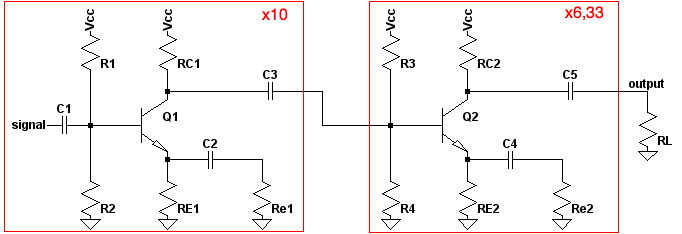
\includegraphics[scale=.6]{teknisk/forforstaerker/blok_forforstaerker.png}
\caption{Blokdiagram over forforstærkerens byggeblokke samt lydsignalets vej}
\label{blok_forforstaerker}
\end{figure}

Udregningerne kan ses i vedlagt pdf (beregning-forforstaerker.pdf). 


\section{Simulering}


\section{Accepttest}

